\documentclass[12pt]{article}
\usepackage{setspace}
\usepackage{geometry}
\usepackage{hyperref}
\usepackage{multicol}
\usepackage{booktabs}
\usepackage{amssymb}
\usepackage{graphicx}
\usepackage{caption}
\usepackage{float}


\geometry{margin=1in}
\bibliographystyle{plain}

\title{Hetergoneity in Lifetime Earnings Risk}

\author{Ethan Ballou\thanks{University of Wisconsin - Milwaukee}}


\date{\today}

\begin{document}
\maketitle
\thispagestyle{empty}


%\date{\today}
%\pubMonth{Month}
%\pubYear{Year}
%\pubVolume{Vol}
%\pubIssue{Issue}
%\JEL{}
%\Keywords{}

\begin{abstract}
\begin{singlespace}
\noindent 
Abstract.  This is our abstract.  It is abstract.  
\end{singlespace}
\end{abstract}
\noindent
\textbf{Keywords}: \\
\textbf{JEL Codes}: \\






\clearpage
\setcounter{page}{1}
\begin{center}
%PRELIMINARY: DO NOT CIRCULATE OR QUOTE
\end{center}




\section{Introduction}

This is an example citation \cite{exampleCitation}.

Multiply all Coefficients by 100?


%\section{Literature Review}

%\section{Data and Model}

%\section{Empirical Strategy}

%\section{Results}

%\section{Conclusion}




%Results \\


























\vspace{4cm}


\begin{figure}[H]
    \centering
    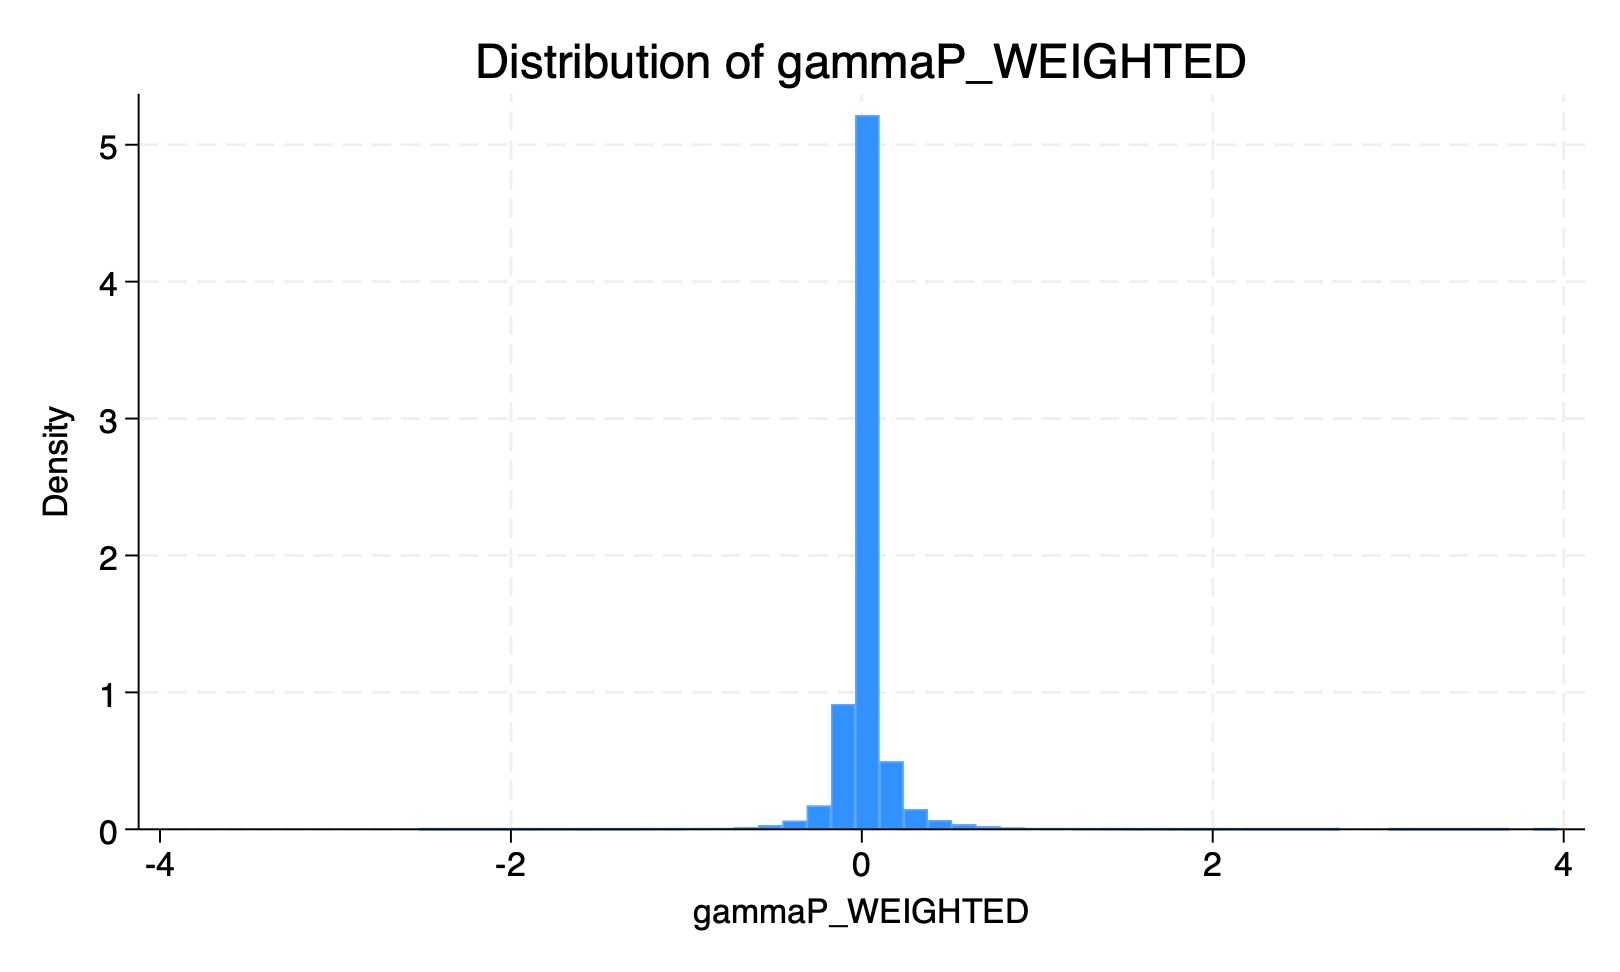
\includegraphics[width=1\textwidth]{/Users/ethanballou/Documents/GitHub/LifetimeEarningsRisk/Plots/histogram_gammaP_WEIGHTED.png}
    \caption{Distribution of gammaP\_WEIGHTED}
\end{figure}



\begin{figure}[H]
    \centering
    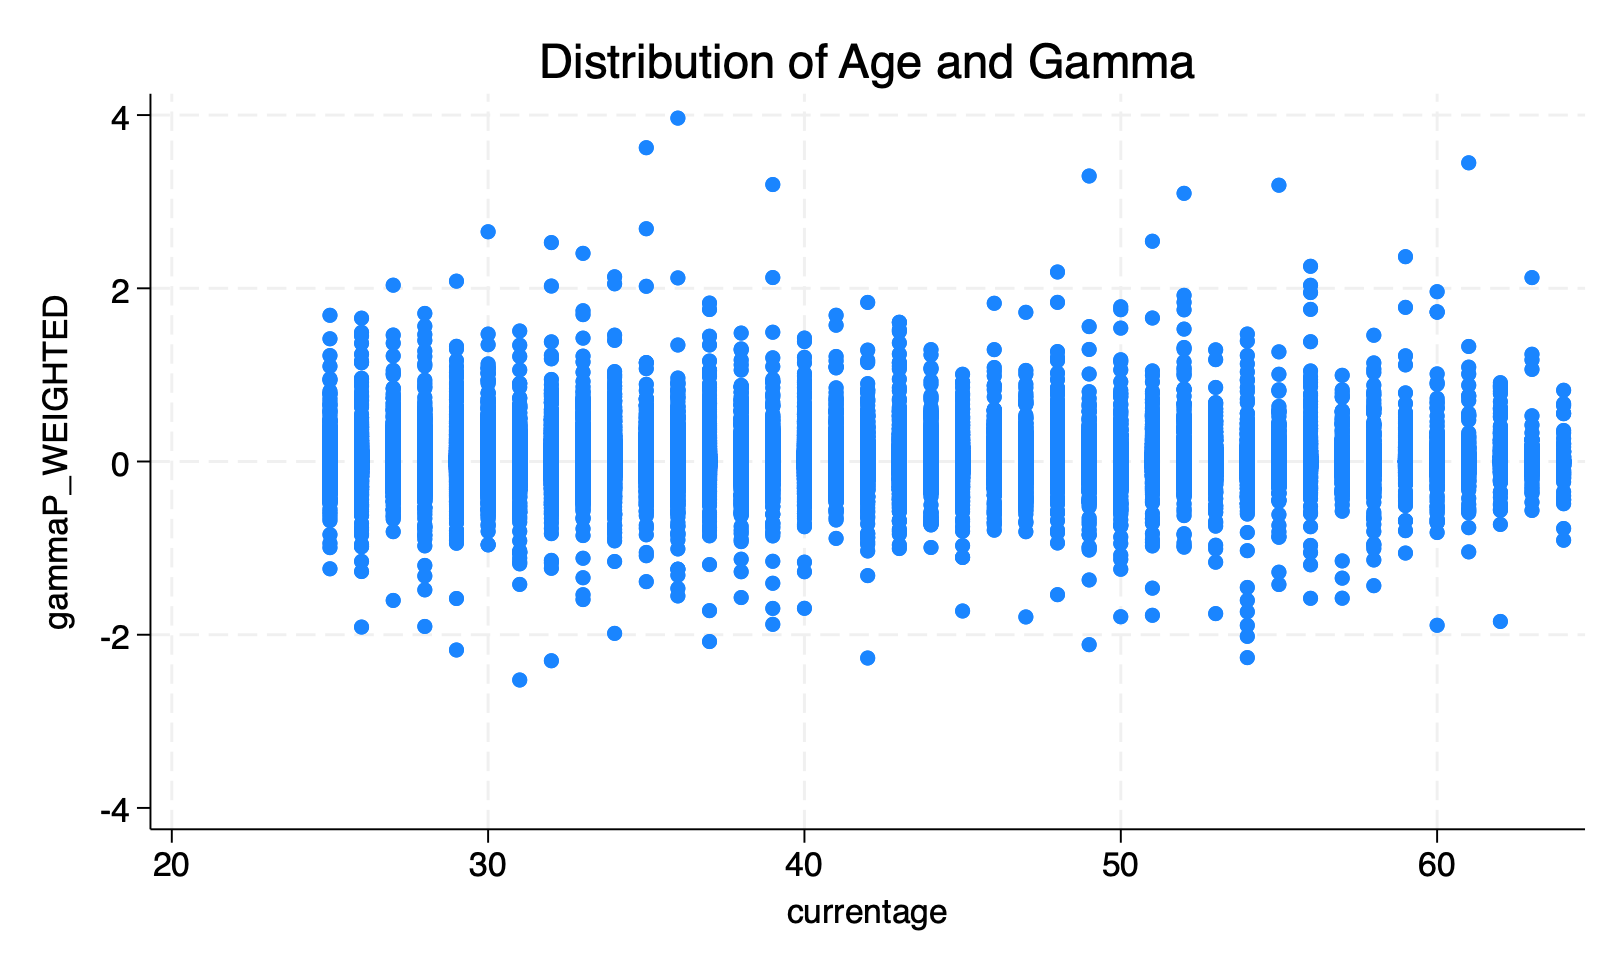
\includegraphics[width=1\textwidth]{/Users/ethanballou/Documents/GitHub/LifetimeEarningsRisk/Plots/scatter_age_gammaP_WEIGHTED.png}
    \caption{Scatterplot of Age vs. gammaP\_WEIGHTED}
\end{figure}






\begin{table}[H]
\centering
\caption{OLS Estimates for $\gamma$ (Coefficients $\times$ 100)}

\begin{tabular}{lccccc}

\toprule
                    & (1)     & (2)   & (3)    & (4)      & (5)         \\
\midrule
EDU1                & $-0.361$  & $-0.360$    & $-0.522^{*}$  & $-0.597^{*}$   & $-0.630^{**}$    \\
                    & (0.255)   & (0.273)     & (0.286)   & (0.307)    & (0.310)     \\
EDU2                & $-0.283$  & $-0.315^{*}$    & $-0.418^{**}$  & $-0.417^{*}$   & $-0.455^{**}$    \\
                    & (0.175)   & (0.181)     & (0.193)   & (0.216)    & (0.219)     \\
EDU3                & $-0.089$  & $-0.063$    & $-0.138$  & $-0.114$   & $-0.147$    \\
                    & (0.206)   & (0.209)     & (0.216)   & (0.228)    & (0.230)     \\
PrRecess            & $-0.006$   & $-0.038$     & $-0.037$   & $-0.040$    & $-0.039$     \\
                    & (0.005)   & (0.036)     & (0.036)   & (0.036)    & (0.036)     \\
rGDPgrow            & $-0.033$   & $0.076$     & $0.071$   & $0.063$    & $0.058$     \\
                    & (0.033)   & (0.172)     & (0.172)   & (0.172)    & (0.172)     \\
fhwage0\_P0         & $-0.006$   & $0.004$     & $0.005$   & $0.002$    & $0.004$     \\
                    & (0.025)   & (0.027)     & (0.027)   & (0.028)    & (0.028)     \\
ma5aep              & $0.004$   & $0.003$     & $0.004$   & $0.004$    & $0.004$     \\
                    & (0.003)   & (0.003)     & (0.003)   & (0.003)    & (0.004)     \\
veteran             & $0.021$   & $-0.003$     & $0.053$   & $0.018$    & $0.040$     \\
                    & (0.141)   & (0.151)     & (0.153)   & (0.154)    & (0.155)     \\
OLF                 & $0.627$   & $0.584$     & $0.550$   & $0.619$    & $0.625$     \\
                    & (0.627)   & (0.628)     & (0.628)   & (0.629)    & (0.629)     \\
tenure              & $-0.010$   & $-0.009$     & $-0.008$   & $-0.012$    & $-0.010$     \\
                    & (0.011)   & (0.012)     & (0.012)   & (0.012)    & (0.012)     \\
currentage          & $0.874^{**}$   & $0.936^{**}$     & $0.926^{**}$   & $0.919^{**}$    & $0.907^{**}$     \\
                    & (0.380)   & (0.384)     & (0.385)   & (0.385)    & (0.385)     \\
currentagesq        & $-0.023^{**}$  & $-0.025^{***}$    & $-0.025^{***}$  & $-0.025^{***}$   & $-0.024^{***}$    \\
                    & (0.009)   & (0.009)     & (0.009)   & (0.009)    & (0.009)     \\
currentagecube      & $0.0002^{***}$  & $0.0002^{***}$    & $0.0002^{***}$  & $0.0002^{***}$   & $0.0002^{***}$    \\
                    & (0.0001)   & (0.0001)     & (0.0001)   & (0.0001)    & (0.0001)     \\

\midrule
Occupation Controls  &               &                 &               & \checkmark    & \checkmark     \\
Industry Controls    &               &                 & \checkmark    &               & \checkmark     \\
Other Controls      &               & \checkmark      & \checkmark    & \checkmark    & \checkmark     \\
\bottomrule
\end{tabular}%
\newline
\textit{Notes:} Standard errors in parentheses. Other controls include state, year, race, and cohort fixed effects. Statistical significance: $^{*}p<0.10$, $^{**}p<0.05$, $^{***}p<0.01$. All coefficients and standard errors are multiplied by 100 for easier interpretation.

\end{table}







\begin{table}[H]
\centering
\caption{Stepwise Results for $\gamma$}

\begin{tabular}{lccccc}

\toprule
                    & (1)     & (2)   & (3)    & (4)      & (5)         \\

\midrule
EDU1                & selected  & 2    & 2  & selected   & selected    \\
EDU2                & selected  & 1    & 1  & selected   & selected    \\
EDU3                & 6  & 10    & 8  & 6   & 6    \\
PrRecess            & 1   & 3     & 3   & 1    & 1     \\
rGDPgrow            & 4   & 4     & 4   & 4    & 4     \\
fhwage0\_P0         & 7   & 11     & 13   & 9    & 9     \\
ma5aep              & 2   & 6     & 6   & 3    & 3     \\
veteran             & 8   & 12     & 12   & 10    & 11     \\
OLF                 & 3   & 5     & 5   & 2    & 2     \\
tenure              & 5   & 7     & 9   & 5    & 5     \\
currentage          & selected   & selected     & selected   & selected    & selected     \\
currentagesq        & selected  & selected    & selected  & selected   & selected    \\
currentagecube      & selected  & selected    & selected  & selected   & selected    \\

\midrule
Occupation Controls      & -   & -    & -  & selected   & selected    \\
Industry Controls      & -  & -    & 7  & -   & 10    \\
Cohort Controls      & -  & 8    & 10  & 7   & 7    \\
Race Controls      & -  & 13    & 14  & 11   & 12    \\
Year Controls      & -  & 9    & 11  & 8   & 8    \\
State Controls      & -  & selected    & selected  & selected   & selected    \\

\midrule
Occupation Controls  &               &                 &               & \checkmark    & \checkmark     \\
Industry Controls    &               &                 & \checkmark    &               & \checkmark     \\
Other Controls      &               & \checkmark      & \checkmark    & \checkmark    & \checkmark     \\

\bottomrule
\end{tabular}%
\newline

\footnotesize
\textit{Notes:} This table reports results from stepwise regression models using a p-value threshold of 0.05. "Selected" indicates variables retained in the final model. Numbers indicate the order of variable removal (with 1 being the last variable removed before model finalization). "-" indicates the variable was not included in the initial model specification.

\end{table}





\begin{table}[H]
\centering
\caption{Lasso Results for $\gamma$}

\begin{tabular}{lccccc}

\toprule
                    & (1)     & (2)   & (3)    & (4)      & (5)         \\

\midrule
EDU1                &  3  &  3    &  2  &  1   &  1    \\
EDU2                &  2  &  1    &  1  &  1   &  1    \\
EDU3                &  8  &  7    &  6  &  6   &  4    \\
PrRecess            &  4    & Not Selected    & Not Selected   & Not Selected    & Not Selected     \\
rGDPgrow            &  6    & Not Selected     & Not Selected   & Not Selected    & Not Selected     \\
fhwage0\_P0         &  7   &  9     &  9   &  8    &  6     \\
ma5aep              &  1   &  2     &  1   &  2    &  1     \\
veteran             &  10   &  8     &  8   &  7    &  5     \\
OLF                 &  3   &  2     &  3   &  1    &  1     \\
tenure              &  5   &  4     &  4   &  3    &  2     \\
currentage          &  9   &  6     &  7   &  5    &  4     \\
currentagesq        &  11  &  10    &  10  &  8   &  7    \\
currentagecube      &  2  &  5    &  5  &  4   &  3    \\

\midrule
Occupation Controls      & -   & -    & -  & Selected   & Selected    \\
Industry Controls      & -  & -    & Selected  & -   & Selected    \\
Cohort Controls      & -  & Selected    & Selected  & Selected   & Selected    \\
Race Controls      & -  & Selected    & Selected  & Selected   & Selected    \\
Year Controls      & -  & Selected    & Selected  & Selected   & Selected    \\
State Controls      & -  & Selected    & Selected  & Selected   & Selected    \\


\midrule
Occupation Controls  &               &                 &               & \checkmark    & \checkmark     \\
Industry Controls    &               &                 & \checkmark    &               & \checkmark     \\
Other Controls      &               & \checkmark      & \checkmark    & \checkmark    & \checkmark     \\

\bottomrule
\end{tabular}%
\newline

\footnotesize
\textit{Notes:} This table reports variables selected by Lasso regression with Bayesian Information Criterion (BIC) variable selection. "Selected" indicates variables retained in the final model. Numbers in parentheses indicate the order in which variables were added to the model. "-" indicates the variable was not included. "Not Selected" indicates the variable was not selected by Lasso but was provided in the model specification.

\end{table}





\begin{table}[H]
\centering
\caption{Lasso and SHAP Results for Occupations}

\scriptsize  % Controls the font size of the table content

\begin{tabular}{lcc|lcc}
\toprule
Occupation & LASSO Order & SHAP Rank & Occupation & LASSO Order & SHAP Rank \\
\midrule
Fisher/Hunter (64) & (1) & (67) & Salesperson (49) & (24) & (54) \\
Aerospace/Marine Engineer (4) & (2) & (17) & Spinner/Weaver (75) & (25) & (64) \\
Music/Perform (17) & (3) & (29) & Bricklay/Carpt (95) & (25) & (19) \\
Dr./Dentist/Vet (6) & (4) & (22) & Bookkeepr/Cash (33) & (26) & (52) \\
Transp. Attend (35) & (5) & (72) & ComputerOperat (34) & (26) & (34) \\
Lumbrman/Axman (73) & (5) & (48) & Rest./StoreMgr (50) & (26) & (39) \\
Prof. Athlete (18) & (7) & (47) & SecurityServic (58) & (26) & (38) \\
Buyer (42) & (7) & (49) & Machine Fitter (84) & (26) & (3) \\
Eng. Tech. Expert (3) & (9) & (44) & Convey. Oper. (97) & (27) & (12) \\
Service Worker (59) & (10) & (35) & Domestic Help (54) & (28) & (41) \\
Farm Manager (61) & (10) & (4) & Forestry Work (63) & (28) & (59) \\
Jewelry Maker (88) & (10) & (60) & RelatMedicalJob (7) & Not selected & (36) \\
Chemist (1) & (13) & (5) & Mathematician (8) & Not selected & (24) \\
Lawyer (12) & (13) & (66) & Cleric (14) & Not selected & (40) \\
Educator (13) & (13) & (13) & Sculptr/Paintr (16) & Not selected & (71) \\
Author (15) & (13) & (45) & Scientist (19) & Not selected & (30) \\
Stenographer (32) & (13) & (46) & Agriculturist (21) & Not selected & (1) \\
Transport. Oper (98) & (13) & (8) & Office Manager (30) & Not selected & (69) \\
Insurance Rep. (44) & (17) & (53) & Administrator (31) & Not selected & (50) \\
Broadcaster (86) & (17) & (56) & Conductor (36) & Not selected & (65) \\
Painter (93) & (17) & (25) & Mailman (37) & Not selected & (9) \\
Tailor (79) & (19) & (20) & Tel. Operator (38) & Not selected & (42) \\
Stat. Mach. Oper (96) & (19) & (41) & Ofc.Worker Etc (39) & Not selected & (55) \\
Architect/Engineer (2) & (20) & (11) & HH Supervisor (52) & Not selected & (77) \\
Vendor (45) & (20) & (10) & Dry-Cleaner (56) & Not selected & (63) \\
Legislator (20) & (21) & (27) & Hair Stylist (57) & Not selected & (75) \\
Tech.Salespers (43) & (21) & (58) & Farm Hand (62) & Not selected & (51) \\
Janitor (55) & (21) & (26) & Inspector (70) & Not selected & (7) \\
Agriculturladm (60) & (21) & (2) & Miner (71) & Not selected & (70) \\
Food Producer (77) & (21) & (37) & Foundry Worker (72) & Not selected & (68) \\
Tool/Die Maker (83) & (21) & (16) & ChemicalWorker (74) & Not selected & (61) \\
Pipe Fitter (87) & (21) & (43) & Shoemaker (80) & Not selected & (62) \\
Labor/Craftsmn (99) & (22) & (18) & Cabinet Maker (81) & Not selected & (73) \\
Accountant (11) & (23) & (15) & Stone Cutter (82) & Not selected & (76) \\
BusinessManagr (40) & (23) & (33) & Electr. Enginr (85) & Not selected & (21) \\
Cook/Waiter (53) & (23) & (28) & Glazier (89) & Not selected & (74) \\
Life/Physical Scientist (5) & (24) & (31) & Printer Etc. (92) & Not selected & (57) \\
Economist (9) & (24) & (14) & Manufacturer (94) & Not selected & (78) \\
& & & Soldier (101) & Not selected & (23) \\
& & & Other (999) & Not selected & (32) \\
\bottomrule
\end{tabular}%
\newline

\footnotesize
\textit{Notes:} This table reports occupations selected by Lasso regression with Bayesian Information Criterion (BIC) for predicting earnings risk. "LASSO Order" indicates the order in which variables would enter the model if the penalty were relaxed. "SHAP Rank" shows the variable importance ranking based on SHAP values (lower numbers indicate greater importance). Note that the BIC-optimal model contained no occupation variables.

\end{table}



\begin{table}[H]
\centering
\caption{Lasso and SHAP Results for Industries}

\begin{tabular}{lcc}

\toprule
Industry & LASSO Selection Order & SHAP Ranking \\
\midrule
Construction (14) & (1) & (7) \\
Other Services (30) & (1) & (4) \\
Clothing/Text. (12) & (3) & (18) \\
Educ./Sport (27) & (3) & (22) \\
Public Admin. (33) & (3) & (10) \\
Chemicals (5) & (6) & (9) \\
Health Service (28) & (6) & (29) \\
Agric.,Forestry (1) & (8) & (20) \\
Other Trans. (21) & (9) & (6) \\
Service Indust (25) & (9) & (21) \\
Postal System (20) & (11) & (24) \\
Mechanical Eng. (9) & (12) & (2) \\
Wood/Paper/Print (11) & (12) & (17) \\
Earth/Clay/Stone (7) & (14) & (16) \\
Volunt./Church (31) & (14) & (28) \\
Wholesale (16) & (16) & (5) \\
Train System (19) & (17) & (3) \\
Insurance (23) & (17) & (25) \\
Electrical Eng. (10) & (19) & (11) \\
Legal Services (29) & (19) & (13) \\
Synthetics (6) & (21) & (23) \\
Volunt./Church (31) & (21) & (28) \\
Food Industry (13) & (23) & (30) \\
Financial Inst. (22) & (24) & (19) \\
Iron/Steel (8) & (25) & (26) \\
Energy/Water (3) & (26) & (1) \\
Mining (4) & (27) & (12) \\
Restaurants (24) & (28) & (27) \\
Other industries & Not selected & Various \\
\bottomrule
\end{tabular}%
\newline

\footnotesize
\textit{Notes:} This table reports industries selected by Lasso regression with Bayesian Information Criterion (BIC) for predicting earnings risk. "LASSO Selection Order" indicates the order in which variables would enter the model if the penalty were relaxed. "SHAP Ranking" shows the variable importance ranking based on SHAP values (lower numbers indicate greater importance). Note that the BIC-optimal model contained no industry variables.

\end{table}







\begin{figure}[H]
    \centering
    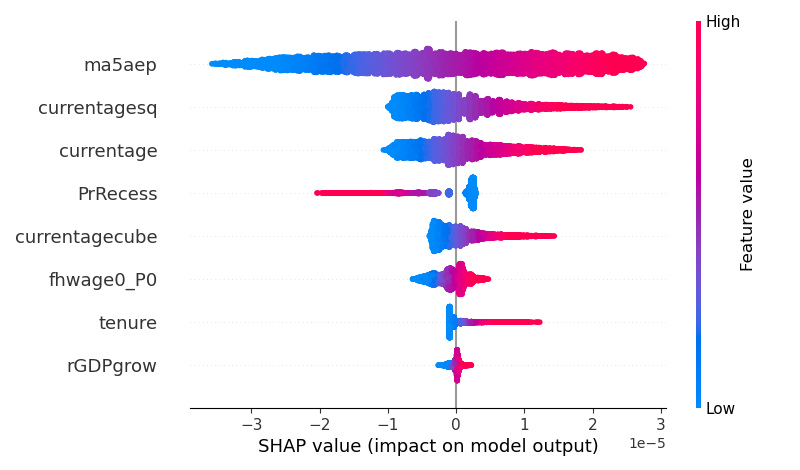
\includegraphics[width=1\textwidth]{/Users/ethanballou/Documents/GitHub/LifetimeEarningsRisk/Plots/ShapSummaryPlot.png}
    \caption{SHAP Summary Plot}
\end{figure}



\begin{figure}[H]
    \centering
    \begin{minipage}{0.49\textwidth}
        \centering
        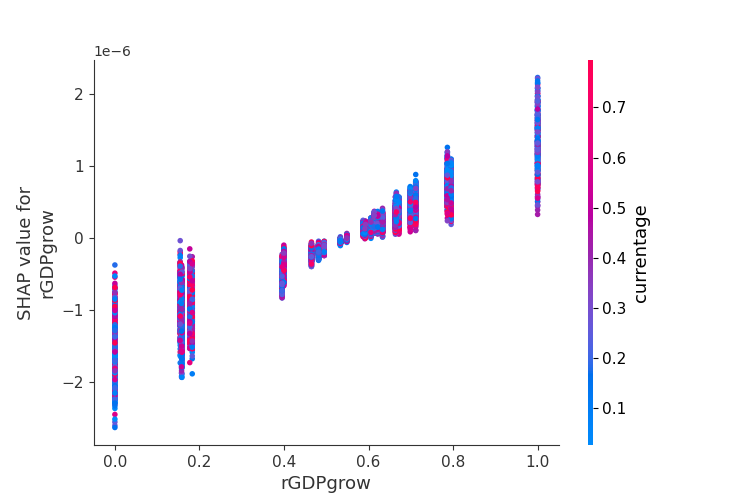
\includegraphics[width=\textwidth]{/Users/ethanballou/Documents/GitHub/LifetimeEarningsRisk/Plots/GDP_Age.png}
        \caption{GDP by Age}
    \end{minipage}
    \hfill
    \begin{minipage}{0.49\textwidth}
        \centering
        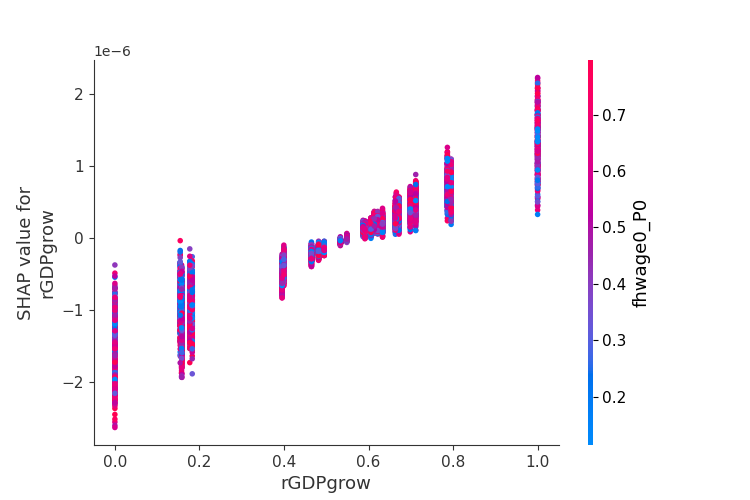
\includegraphics[width=\textwidth]{/Users/ethanballou/Documents/GitHub/LifetimeEarningsRisk/Plots/GDP_Income.png}
        \caption{GDP by Income}
    \end{minipage}
\end{figure}






\bibliography{references}

\end{document}